

\chapter{Numerical Solution of Drift-Diffusion Equation} % Main chapter title

\label{Chapter3} % Change X to a consecutive number; for referencing this chapter elsewhere, use \ref{ChapterX}

\lhead{Chapter 3. \emph{Numerical Solution for Drift-Diffusion Equations}} % Change X to a consecutive number; this is for the header on each page - perhaps a shortened title

%----------------------------------------------------------------------------------------
%	SECTION 1
%----------------------------------------------------------------------------------------

\section{Finite Difference Method}
There are many different methods that can be used to solve drift diffusion equations such as finite elements, finite difference or meshless methods. We will be using finite difference method which uses an approximation for the derivative of a function based on the mathematical definition of the derivative.

\begin{equation}
\frac{df}{dx}=\lim\limits_{h \rightarrow 0} \frac{f(x+h)-f(x)}{h}
\end{equation}

We can get a numerical approximation for the first derivative by dropping the limit and assuming that h is small enough to get a value for the derivative reasonably close to the actual value. Of course as h gets smaller the approximation becomes more and more accurate. The difference between the calculated value and the real value is called the truncation error and it is captured using $O(h^n)$ notation. n signifies the order of h which determines how fast the approximation is approaching the real solution as h decreases.  
\begin{equation}
\frac{df}{dx}=\frac{f(x+h)-f(x)}{h} + O(h)
\label{numdif}
\end{equation}

It is possible to uniformly discretise the entire region over which a function is defined in order to calculate its derivative. We start by dividing the region over which the function is defined into \textit{n-1} segments therefore there will be \textit{n} number of points. Then we can find the length of each segment using the following relationship:

\begin{equation}
h=\frac{L}{n}
\end{equation}

The function we are interested in is defined on the edge of every segment. We can label each point consecutively, $x_0,x_1,x_2$ ... $x_{n-1}$ where $x_i=ih$. Our function is discretely defined on \textit{$f_{i}=f(x_{i})$} where\textit{ i=0,1,2..n-1}. It is possible to use equation  \ref{numdif} to discretely calculate the first derivative of the function with respect to x.

\begin{equation}
\frac{df(x_i)}{dx}=\frac{f(x_{i+1})-f(x_i)}{h} + O(h)
\end{equation}
Above equation is called forward difference because the derivative for point $x_i$ was calculated using the point that is coming right after it, $x_{i+1}$.
\begin{equation}
f^{'}_i=\frac{f_{i+1}-f_i}{h}+ O(h)
\end{equation}

Forward difference is not the only way to calculate a discrete derivative. Here are a few more ways calculate the same derivative by making use of different points.

\begin{equation}
f^{'}_i=\frac{f_{i}-f_{i-1}}{h}+ O(h)
\label{bdif}
\end{equation}

\begin{equation}
f^{'}_{i+\frac{1}{2}}=\frac{f_{i+1}-f_i}{h}+ O(h^2)
\label{cdif}
\end{equation}

Equation \ref{bdif} is called backward difference and equation \ref{cdif} is called central difference. One important thing to note here is that in the central difference formula the derivative falls exactly in the middle of two points. It also gives more accurate results using the same number of points as forward and backward difference. 

Using finite difference formulas it is possible to construct higher derivatives. Lets look at how to get a formula for a second order derivative at point $x_i$ using central difference. First step is to calculate the first order derivative on $x_{i-\frac{1}{2}}$, $x_i$ and $x_{i+\frac{1}{2}}$  

\begin{equation}
f_{i+\frac{1}{2}}^{'}=\frac{f_{i+1}-f_{i}}{h}
\label{forwardd}
\end{equation}

\begin{equation}
f_{i-\frac{1}{2}}^{'}=\frac{f_{i}-f_{i-1}}{h}
\end{equation}

\begin{equation}
f^{'}_{i}=\frac{f_{i+\frac{1}{2}}-f_{i-\frac{1}{2}}}{h}
\end{equation}

We can take the second derivative of the last function and plug in the first two.

\begin{equation}\nonumber
f^{''}_{i}=\frac{f_{i+\frac{1}{2}}^{'}-f_{i-\frac{1}{2}}^{'}}{h}
\end{equation}

\begin{equation}\nonumber
f^{''}_{i}=\frac{\frac{f_{i+1}-f_{i}}{h}-\frac{f_{i}-f_{i-1}}{h}}{h}
\end{equation}

\begin{equation}\nonumber
f^{''}_{i}=\frac{f_{i+1}-f_{i}-f_{i}+f_{i-1}}{h^2}
\end{equation}

After some algebra we get the final form of the second derivative.
\begin{equation}
f^{''}_{i}=\frac{f_{i+1}-2f_{i}+f_{i-1}}{h^2}+O(h^2)
\label{fdc2}
\end{equation}

Overall these finite difference equations are enough to solve drift diffusion equations. Even though all the derivations were done in 1-D it is trivial to extend them to higher dimensions. Now we can use finite difference method to solve Poisson's equation and drift diffusion equations.

\clearpage
\section{Solving Drift-Diffusion Equations}
\subsection{Poisson Solver}

Since we are dealing with electronic devices there is usually going to be an electric field in the system generated by an external source or generated within the device through charged particles. Either way we need to solve Poisson's equation in order find the potential distribution as well as the electric field inside the device. We can start by simplifying the equation through assumptions and then we can employ finite difference to solve this simplified equation. The first step of simplification is assuming that the permittivity is isotropic, then we can get: 
 
\begin{equation}
\nabla \cdot  (\varepsilon \nabla V)=-\rho
\end{equation}

\begin{equation}
\nabla \cdot  (\varepsilon \nabla V)=\varepsilon  \nabla^2 V
\end{equation}

We can also move the permittivity to the right hand side and get,

\begin{equation}
 \nabla^2 V =-\frac{\rho}{\varepsilon}
\end{equation}

Expanding the left hand side,
\begin{equation}
 \nabla^2 V =\frac{\partial^2 V}{\partial^2 x}+\frac{\partial^2 V}{\partial^2 y}
\end{equation}

After discretizing electric potential over a 2-D uniform grid and using the second order central finite difference formula \eqref{fdc2} we get the following equation,

\begin{equation}
 \nabla^2 V_{i,j}=\frac{V_{i+1,j}-2V_{i,j}+V_{i-1,j}}{\Delta x^2}+\frac{V_{i,j+1}-2V_{i,j}+V_{i,j-1}}{\Delta y^2}
\end{equation}

Since the grid is uniform we can use the same value for the distance between the nodes in each direction.

\begin{equation}
\Delta=\Delta x =\Delta y
\end{equation}

Of course the net charge density and the permittivity is also discretized over the same uniform mesh. Putting all this information together we have generated a numerical approximation for Poisson's equation. 

\begin{equation}
 \nabla^2 V_{i,j}=\frac{V_{i-1,j}+V_{i,j-1}-4V_{i,j}+V_{i+1,j}+V_{i,j+1}}{\Delta^2}=-\frac{\rho_{i,j}}{\varepsilon_{i,j}}
\end{equation}

If we rearrange this equation by keeping all the known values on the right hand side and all the unknown values on the left hand side we get the following equation.
\begin{equation}
\varepsilon_{i,j}(V_{i-1,j}+V_{i,j-1}-4V_{i,j}+V_{i+1,j}+V_{i,j+1})=-\Delta^2\rho_{i,j}
\label{discrete_poisson}
\end{equation}

Above equation is valid for almost all the nodes in the system except two cases, boundary nodes and interface nodes. We can have two different types of boundary conditions which determine how the boundaries are going to be handled. The first one is Dirichlet boundary condition which forces a particular value for the potential at the boundary.

\begin{equation}
V_{i,j}=V_{b}
\label{dirichlet}
\end{equation}

Where $V_{b}$ is the value of the potential at the boundary. The other possible boundary condition is called Neumann boundary condition which states that the derivative of the potential at the boundary is zero. This gives us the following equation:

\begin{equation}
\frac{\partial V}{\partial x}=\frac{V_{i+1,j}-V_{i,j}}{\Delta}=0
\end{equation}

So for a boundary over y axis we get:
\begin{equation}
V_{i+1,j}=V_{i,j}
\end{equation}

Following the same procedure we can get Neumann boundary condition over x axis:
\begin{equation}
V_{i,j+1}=V_{i,j}
\end{equation}
After we have handled all the boundary conditions we have to figure out how to handle interfaces. These interfaces occur when two materials with different permittivities come into contact. So when we have a node at the interface the permittivity of that node is ambiguously defined. We need a special way to solve this ambiguity. It is possible to derive a finite difference equation that handles dielectric interfaces properly starting from Gauss's Law.
\begin{equation}
\oint \varepsilon \vec{E} \cdot \vec{ds}=Q
\end{equation}
After piecewise integration around the boundary we can get an equation for a horizontal interface and a vertical interface respectively:
\begin{equation}
(\varepsilon_1+\varepsilon_2)V_{i-1,j}+(\varepsilon_1+\varepsilon_2)V_{i+1,j}-4(\varepsilon_1+\varepsilon_2)V_{i,j}+2\varepsilon_1 V_{i,j+1}+2\varepsilon_2 V_{i,j-1}=Q_{i,j}=\Delta^2\rho_{i,j}
\label{inth}
\end{equation}

\begin{equation}
(\varepsilon_1+\varepsilon_2)V_{i,j-1}+(\varepsilon_1+\varepsilon_2)V_{i,j+1}-4(\varepsilon_1+\varepsilon_2)V_{i,j}+2\varepsilon_1 V_{i+1,j}+2\varepsilon_2 V_{i-1,j}=Q_{i,j}=\Delta^2\rho_{i,j}
\label{intv}
\end{equation}

Now that we have all the equations we need for all the nodes over the simulation domain it is possible to combine them (\eqref{discrete_poisson},\eqref{dirichlet},\eqref{inth}, \eqref{intv}) into a matrix and turn Poisson's equation, which is a second order differential equation, into a linear equation.

\begin{equation}
D_{2}\vec{V}=-\Delta^2\vec{\rho}-\vec{V_b}
\end{equation}

One can easily get the potential distribution by simply solving the matrix equation obtained. Due to the nature of the problem the matrix we end up with is quite sparse and using a sparse LU decomposition dramatically increases the computational efficiency.

\begin{equation}
\vec{V}=D_{2}^{-1}(-\Delta^2\vec{\rho_{i,j}}-\vec{V_b})
\end{equation}

After solving for the potential distribution it is easy to calculate the electric field distribution discretely using the relationship between electric field and electric potential \eqref{Efield} and central difference equation \eqref{cdif}. 

\begin{equation}
\vec{E^x_{i,j}}=-\frac{V_{i+1,j}-V_{i-1,j}}{2\Delta}
\end{equation}

\begin{equation}
\vec{E^x_{i,j}}=-\frac{V_{i,j+1}-V_{i,j-1}}{2\Delta}
\end{equation}

\clearpage
\subsection{Current Density Equations}
After we have calculated the electric field distribution over the entire region we can now figure out how the particles move. Both drift and diffusion currents can be calculated over the entire grid. There are few different methods that can be used to calculate the current density. The accuracy of the methods we will look at change based on the physics of the device.
\subsubsection{Finite Difference Method}
The first method involves simply applying finite difference to calculate drift and diffusion currents. Drift current is quite simple since it does not involve any differentials and the diffusion current can be calculated using first order central difference. The current density is calculated in such a way that it falls between two points which simplifies the application of the boundary conditions.
\begin{equation}
J^x_{i+\frac{1}{2},j,k}=q\mu_n n_{i+\frac{1}{2},j,k} E^x_{i+\frac{1}{2},j,k}+D_n \frac{n_{i+1,j,k}-n_{i,j,k}}{\Delta}
\end{equation}
The electric field was calculated exactly on the nodes but we can use linear interpolation in order to get a value between the nodes. Same argument is also valid for particle densities \textit{p} and \textit{n}. They were defined on the nodes but can be linearly interpolated.

\begin{equation}\nonumber
n_{i+\frac{1}{2},j,k}=\frac{n_{i+1,j,k}+n_{i,j,k}}{2}
\end{equation}
\begin{equation}\nonumber
E^{x}_{i+\frac{1}{2},j,k}=\frac{E^y_{i+1,j,k}+E^y_{i,j,k}}{2}
\end{equation}

We can follow the same method in order to calculate the current density in y direction:
\begin{equation}
J^y_{i,j+\frac{1}{2},k}=q\mu_n n_{i,j+\frac{1}{2},k} E^y_{i,j+\frac{1}{2},k}+D_n \frac{n_{i,j+1,k}-n_{i,j,k}}{\Delta}
\end{equation}
\begin{equation}\nonumber
n_{i,j+\frac{1}{2},k}=\frac{n_{i,j+1,k}+n_{i,j,k}}{2}
\end{equation}
\begin{equation}\nonumber
E^{y}_{i,j+\frac{1}{2},k}=\frac{E^y_{i,j+1,k}+E^y_{i,j,k}}{2}
\end{equation}

Same current density equations can be used for positively charged particles by replacing n by p and changing the sign of the diffusion term.


\subsubsection{Boundary Conditions}

For a drift diffusion problem there are two different possibilities for boundary conditions. The first one is when the particles cannot go past through a certain boundary, no flow boundary condition. This can be achieved by using Dirichlet bounday condition and setting the flow at the boundary to zero. 
\begin{equation}
J=0
\end{equation}

This boundary condition can also be used conditionally. A straightforward example is when there is a particle density limit over an area. This condition can be used to cut the flow of particles into an area when a certain particle concentration is reached. 

Dirichlet boundary condition can also be used in cases where there is a flow through the boundary. A good example is a metal contact. It is assumed that metal contact has infinite amount of charge and the boundary is always charge neutral. For example if we have holes, electrons, positive and negative doping we can assume that at the boundary positive charge concentration will be equal to the negative charge concentration. 

\begin{equation}
N_{D} + p=N_{A} + n
\label{chargeneutrality}
\end{equation}

If we are dealing with a semiconductor the amount of holes and electrons has to obey mass action law at equilibrium.

\begin{equation}
np=n_i^2
\label{massaction}
\end{equation}

$n_i$ here is the concentration of the semiconductor at equilibrium before getting doped. Solving \eqref{massaction} and \eqref{chargeneutrality} together we get,

\begin{equation}
n=\frac{1}{2}(N_D - N_A + \sqrt{(N_D - N_A)^2+4n_i^2})
\label{nbound}
\end{equation}

We can calculate the hole concentration using mass action law.

\begin{equation}
p=\frac{n_i^2}{n}
\label{pbound}
\end{equation}

So we have a Dirichlet condition for electrons and hole which are given by \ref{nbound} and \ref{pbound} respectively.

\clearpage
\subsection{Continuity Equation}
Continuity equation is needed to calculate a transient solution for drift diffusion equations. The equation is simple to discretize using finite difference method. There are two terms that need to be discretized, a first order derivative in time and space. We can first start by evaluating the divergence term in equation \eqref{conn}.

\begin{equation}
\nabla \cdot J=\frac{\partial J}{\partial x}+\frac{\partial J}{\partial y}=\frac{d J_x}{d x}+\frac{d J_y}{d y}
\end{equation}

It is possible to replace the derivative with central finite difference terms.
\begin{equation}
\frac{d J_x}{d x}=\frac{J^x_{i+\frac{1}{2},j,k}-J^x_{i-\frac{1}{2},j,k}}{h}
\end{equation}
\begin{equation}
\frac{d J_y}{d y}=\frac{J^y_{i,j+\frac{1}{2},k}-J^y_{i,j-\frac{1}{2},k}}{h}
\end{equation}
\begin{equation}
\nabla \cdot J_{i,j,k}=\frac{J^x_{i+\frac{1}{2},j,k}-J^x_{i-\frac{1}{2},j,k}}{h}+\frac{J^y_{i,j+\frac{1}{2},k}-J^y_{i,j-\frac{1}{2},k}}{h}
\end{equation}

This is the general form of the divergence of the current density. We can plug in the current density equations from either finite difference or Scharfatter-Gummel approach. Collecting everything in a matrix gives rise to the following equation:

\begin{equation}
\nabla \cdot J_k =B
\label{fd_div}
\end{equation}

The time derivative can also be replaced by a forward or backward finite difference terms respectively.

\begin{equation}
\frac{\partial  \vec{n}_k}{\partial t}=\frac{ \vec{n}_{k+1}-\vec{n}_k}{\Delta t}
\label{forwardtime}
\end{equation}

\begin{equation}
\frac{\partial \vec{n}_k}{\partial t}=\frac{ \vec{n}_k- \vec{n}_{k-1}}{\Delta t}
\label{backwardtime}
\end{equation}

It is possible to find a numerical transient solution for the drift-diffusion problem by combining finite difference form of the time derivative (\eqref{forwardtime} or \eqref{backwardtime}) and the divergence of the current density equations \eqref{fd_div}.

Using forward difference approximation we get,

\begin{equation}\nonumber
\frac{ \vec{n}_{k+1}-\vec{n_k}}{\Delta t}=B
\end{equation}

\begin{equation}
\vec{n}_{k+1}=\vec{n_{k}}+\Delta t B
\label{explicit}
\end{equation}

Both forward and backward difference formulas work sequentially in order to generate a transient solution. In order to calculate the next time step we need the solution of the previous time step. Forward difference gives us an explicit solution which has few advantages. This solution can be implemented without forming any matrices, just by directly calculating the divergence of the current density for each node and then marching through time using equation \ref{explicit}. Additionally, unlike backward difference, there are no equations to be solved for every time step. These two properties ease the computational load of the problem and speed up the solution process. Unfortunately this scheme has very strict stability conditions which has to be met in order to get a reasonable solution.

Using backward difference approximation we get,
\begin{equation}\nonumber
\frac{ \vec{n}_{k}-\vec{n}_{k-1}}{\Delta t}=\frac{1}{q}(qB)
\end{equation}
\begin{equation}\nonumber
\vec{n}_{k}-\Delta t B =\vec{n}_{k-1}
\end{equation}

Since all the equations in B matrix are linear we can pull $n$ out $(B=Cn)$ and rearrange the equation.
\begin{equation}\nonumber
\vec{n}_{k}-\Delta t C\vec{n}_{k-1} =\vec{n}_{k-1}
\end{equation}
\begin{equation}
\vec{n}_k=(I-\Delta t C)^{-1}\vec{n}_{k-1}
\end{equation}

Now we have an implicit solution which seem quite similar to the previous solution but in fact they are quite different. This solution needs a matrix inversion every time step but it is unconditionally stable. The decision to use implicit or explicit solution is not very simple and it will be discussed in detail the next section.
\clearpage
\subsection{Stability and Computational Efficiency}
Before we go into numerical limitations of solving drift diffusion equation via finite difference we should look into physical limitations of the problem. These limitations persist no matter what kind of numerical scheme is employed to solve drift diffusion equations.

\subsubsection{Physical Limitations}
Debye length is the length over which mobile charge carriers screen out an external electric field. It determines how steeply charges will accumulate over a certain distance when subject to an electric field. 
\begin{equation}
L_D=\sqrt{\frac{\varepsilon V_{th}}{q n}}
\label{debye}
\end{equation}
Debye length limits how coarse the grid can be since we need to be able to accurately capture the distribution of charge density. As it can bee seen from the formula above the higher the charge density is the steeper the charge will accumulate. This can become a major problem for device sizes in millimetre range or higher and high charge concentrations since the mesh density needs to be extremely high.

The amount if time it takes for charge fluctuations to disappear is called Dielectric relaxation time. It limits the maximum time step of a simulation since the fluctuations that are not properly resolved over time will make the simulation unstable.

\begin{equation}
t_{dr}=\frac{\varepsilon}{q n \mu}
\label{tdr}
\end{equation}

Dielectric relaxation time is only important when electric potential is highly affected by redistribution of charge over time. Otherwise it has minimal impact on the stability of the problem.
\subsubsection{Numerical Limitations}

There are also numerical limits which can affect convergence and stability of a solution when using an explicit scheme. These are called Courant-Friedrichs-Lewy (CFL)conditions. We can look at CFL conditions for pure diffusion and pure drift.

\begin{equation}
\frac{\Delta ^2}{2 D_n}>\Delta t
\label{CFL_Diff}
\end{equation}

Above condition is for pure diffusion and it restricts the maximum time step. Following condition is for drift dominated systems:

\begin{equation}
\frac{2 \Delta }{\mu E}>\Delta t
\label{CFL_Drift}
\end{equation}

This is the second numerical restriction on our simulation. Interestingly the condition for drift depends on the electric field therefore it needs to be satisfied as the electric field changes over time during simulation.

Now we have all the conditions we need to ensure the stability of the simulation. Both physical and numerical constraints have to be evaluated and mesh density and time step need to be selected in order to satisfy all these conditions discussed above. Particularly mesh density have a very strong effect on the accuracy, stability and computational efficiency of the simulation. Increasing mesh density increases the computational time needed to calculate every time step since we have more points. Additionally because of the CFL condition for diffusion time step is related to the square of the mesh size. This means that maximum allowed step size decreases much quicker than the mesh density. Also, increasing charge density can decrease the maximum mesh size to a very small value. This can be somewhat fixed by using a non uniform mesh which can dramatically decrease the amount points needed for the simulation. Unfortunately this is usually not very straightforward to implement in a finite difference scheme. 

\subsubsection{Explicit vs. Implicit Solution}

Overall explicit and implicit solutions have their advantages and disadvantages. Choosing one over the other requires careful analysis of the problem. Implicit solution by itself is unconditionally stable therefore it can support very large time steps without any stability issues. However with increased time step, the accuracy of the transient solution decreases but the steady state solution does not get affected. So for steady state solutions it is better to use an implicit method which can reach steady state very quickly. This advantage disappears when particle densities are high enough to affect the electic field and Poisson's equation needs to be solved for every time step. In this scenario the maximum step size is determined by dielectric relaxation time which tends to be around the same order as CFL conditions. Now since the time step is going to be around the same order for both implicit and explicit methods it makes sense to use the explicit one because it is computationally less expensive.

We can sum this brief analysis by stating that implicit solution is preferable when there is no coupling between Poisson's equation and drift diffusion equations and the transient response is not very important. Explicit solution have an edge over the implicit solution due to its lower computational resource requirement when the equations are coupled and the time steps for both schemes are restricted to fairly small values. 

\clearpage
\subsection{Simulation Procedure}
Over the past section we have gone through different equations and schemes that are used to solve drift diffusion and Poisson's equation. Using all this information we can create a general strategy to solve a drift diffusion problem. 

First of all we need to define the geometry and physical properties of the problem as well as all initial and boundary conditions. Initialization sets up the first time step of the problem at $t=0$. Once this first step is done we can generate required vectors and matrices and solve the problem for the next time steps, $t=t_i$. 

The solution process starts by solving Poisson's equation using the charge distribution at current time step. Once it is solved we can calculate the electric field distribution and use it in drift diffusion equations to calculate current density distribution. One important choice to make here is to either use finite difference method or Scharfatter-Gummel method in order to calculate current density. The conditions that favor one or the other are not simple to determine and will be discussed in detail in the next chapter. The next decision to be made is either to use an implicit or explicit solution which will determine if we can directly calculate the next step or need to solve a matrix. Finally once we have the carrier distribution for the next step we can check for a stopping criterion. If this criterion is not met then the whole process will start all over again with a small difference. If the charge concentration is so small that the equations are decoupled then we can skip solving Poisson's equation again. This can significantly speed up the simulation since we only need to solve for the continuity equation after this point.

 There are two different criteria that can be used to decide weather to finish the simulation or not. We can stop if we intend to solve for a certain time frame and we reached the final time. This is quite simple since we look at the current time and if it is equal or greater than the required simulation time we can just stop the simulation. We could also be interested in reaching a steady state solution. This can be determined by comparing the current carrier distributions with distribution at the previous time step. If the difference is very small then we can conclude that the simulation has reached steady state and it is time stop the solution process. This makes physical sense since it makes sure that the time derivative of the carrier densities are close to zero. The flowchart in figure \ref{flowchart} summarizes the solution procedure.


\clearpage

\begin{figure}
\centering
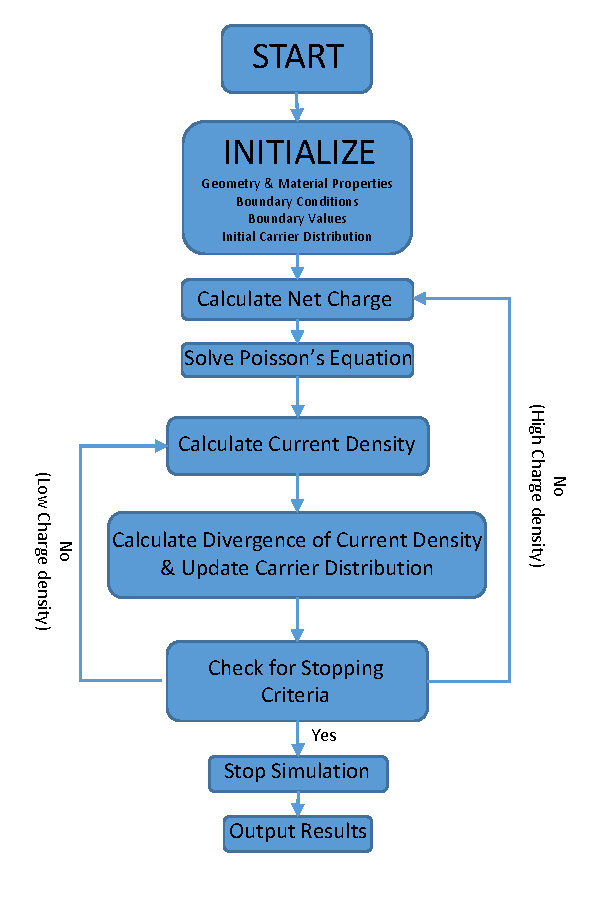
\includegraphics[scale=1.3]{flowchart}
\caption{Finite Difference Drift-Diffusion Scheme Flowchart} 
\label{flowchart}
\end{figure}
